\chapter{Analysis of Parasite Clearance Times}
The derived PC90 values using the log-linear interpolation method are shown in Table \ref{derivedPC90}
\begin{table}[h]
\centering
\caption{Derived PC90 values in hours}\label{derivedPC90}
\begin{tabular}{|cc|c|c|}
\hline
&&\multicolumn{2}{c|}{Treatment}\\
&&alone&combined\\\hline
\multirow{2}{*}{Centre 1}&Male&$\begin{array}{c}3.85,\ 27.32,\ 36.30,\  8.84,\\4.35,\  1.53,\ 30.01,\  4.83\end{array}$&$\begin{array}{c}9.47,\  5.05,\  8.10,\\22.77,\  9.40,\  7.73\end{array}$\\\cline{2-4}
&Female&$\begin{array}{c}19.76,\ 22.45,\\21.75,\ 46.52\end{array}$&$\begin{array}{c}3.65,\ 8.40 ,\ 9.69,\\0.85,\ 9.04,\ 9.38\end{array}$\\\hline
\multirow{2}{*}{Centre 2}&Male&$\begin{array}{c}4.82,\ 2.21,\\11.59,\ 28.09\end{array}$&$\begin{array}{c}17.15,\ 9.51,\\14.68,\ 8.08\end{array}$\\\cline{2-4}
&Female&$\begin{array}{c}21.97,\ 2.49,\ 25.08,\ 31.63,\\5.00,\ 21.64,\ 24.42\end{array}$&$\begin{array}{c}14.77,\  8.75,\\5.84,\ 6.23\end{array}$\\\hline
\end{tabular}
\end{table}
\section{Graphical comparison}
The PC90 data from Table \ref{derivedPC90} are plotted by experimental factors centre, sex and treatment in Figure \ref{pc90boxes}, summarised in two ways. Firstly, by the median and upper and lower quartiles. Secondly, the mean is shown with 95\% confidence intervals from the $t$ distribution defined by the standard error of the data\footnote{The $t$ distribution confidence intervals are calculated using the \texttt{smean.cl.normal} \emph{R} functions from the Hmisc library\cite{Hmisc}}. These confidence intervals for the mean are relevant for parametric tests based on the normal distribution such as ANOVA and give an indication of differences that may be significant.
\begin{figure}[p]
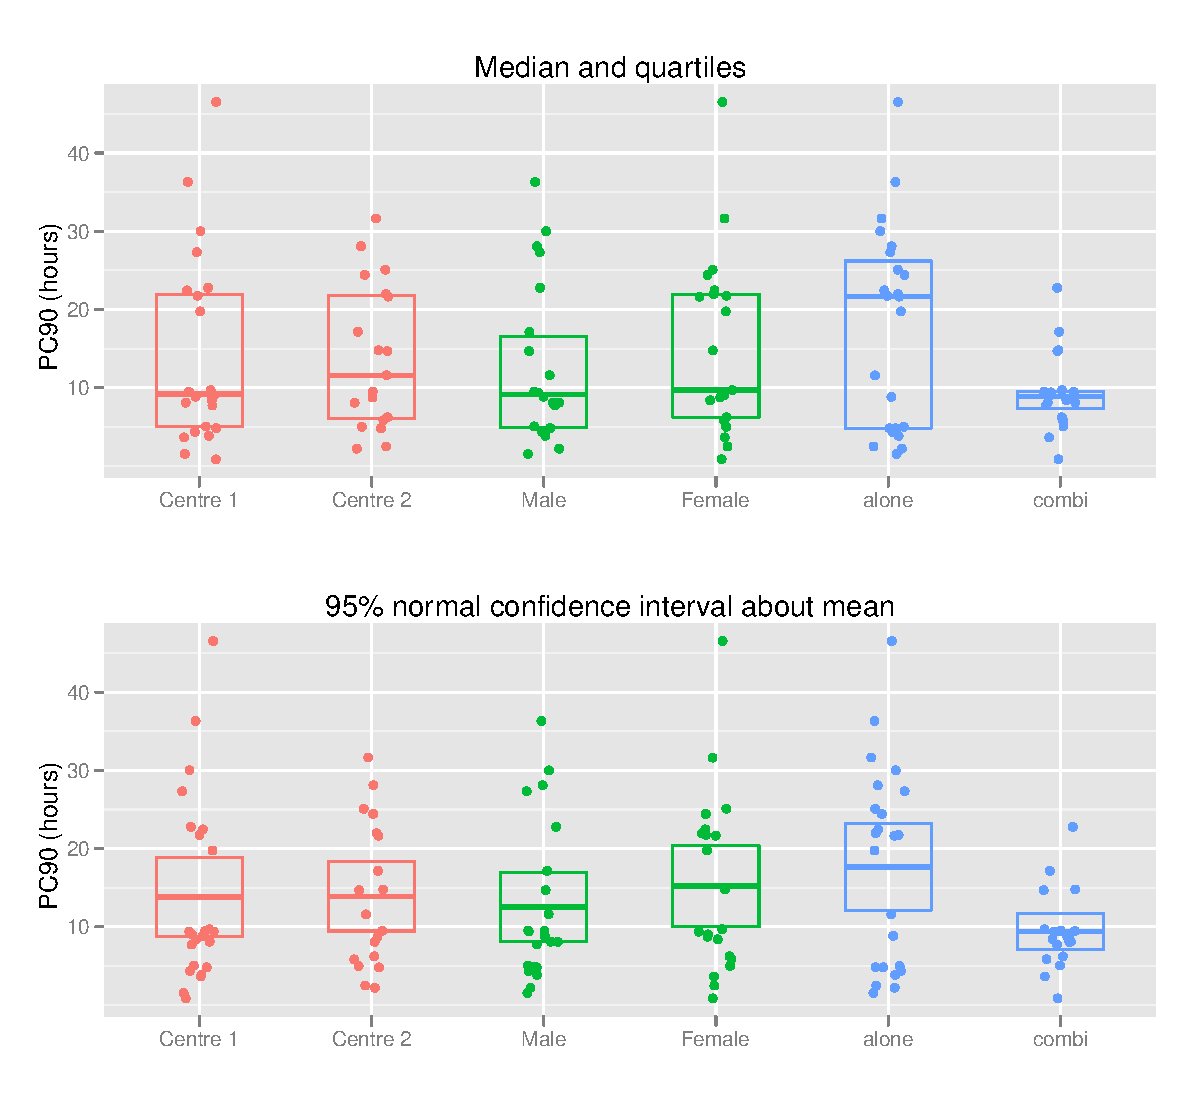
\includegraphics[width=6.5in]{pc90boxes.eps} 
\caption{Comparison of PC90 by experimental factors with medians and quartiles and $t$ distribution 95\% confidence intervals for the means}
\label{pc90boxes}
\end{figure}

It can be seen in Figure \ref{pc90boxes} that there doesn't seem to be any notable difference in clearance times between centres. Female subjects seem to have a larger variance in clearance times and perhaps a slightly longer clearance time on average. The difference in clearance times due to the treatment chosen seems to have the largest influence with a larger spread in clearance times for subjects on the ``alone'' single-drug treatment with a potentially significant decrease in mean clearance time for the subjects on the combined-drug treatment.

An additional observation is that the distributions seem bimodal in the cases of the Centre 1, Female and alone subjects. LOOK AT RAW PLOTS TO SEE WHAT IS GOING ON.

In Figure \ref{pc90interaction} the data is split two ways in each plot to look for interaction effects betwee the factors. Again, the mean and 95\% confidence intervals for the mean are shown.
\begin{figure}[p]
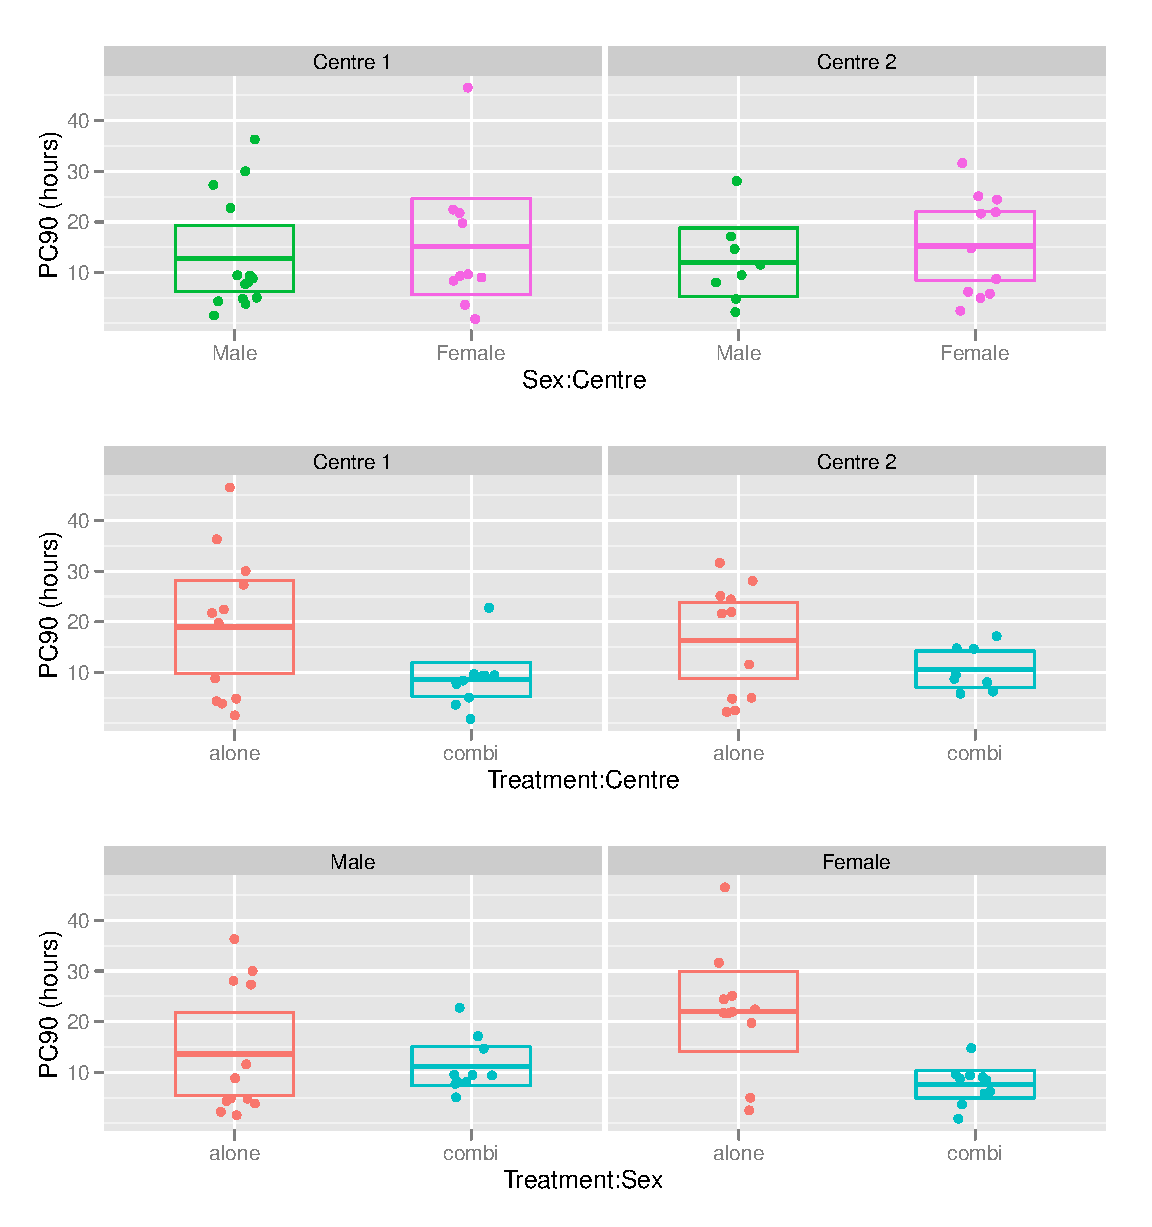
\includegraphics[width=6.5in]{pc90interaction.eps} 
\caption{PC90 two-way interactions with 95\% confidence intervals for the means}
\label{pc90interaction}
\end{figure}

It can be seen that there doesn't seem to be any interaction between sex and centre or treatment and centre i.e. the left and right panels of the top two plots look essentially the same. However, it appears that the combined treatment only decreases the mean clearance time for female subjects.
\section{ANOVA modelling by experimental factors}
3-way ANOVA with all interactions was performed on the PC90 data in Table \ref{derivedPC90}. The fitted model is
\begin{equation}
\mathrm{PC}90_{ijkl}=\mu+C_i+S_j+T_k+(CS)_{ij}+(CT)_{ik}+(ST)_{jk}+(CST)_{ijk}+\epsilon_{ijkl}\quad\quad\epsilon\sim N(0,\sigma^2)\label{full}
\end{equation}
where PC$90_{ijkl}$ is the clearance time for subject $l$ in centre $i$, of sex $j$ on treatment $k$; $C_i$ is the effect of the centre, $S_j$ the effect of the sex; $T_k$ the treatment effect; $CS_{ij}$ the interaction effect of centre and sex and so on ($i,j,k=1,2$). Using a corner-point constraint, $\mu$ corresponds to $E[\mathrm{PC}90]$ for a centre 1, male on the single-drug treatment, with all other terms in the model representing the difference from this mean.

The standardized residuals ($e/\hat{\sigma}$) obtained from fitting model \ref{full} are plotted in Figure \ref{aovloglinres}.
\begin{figure}[p]
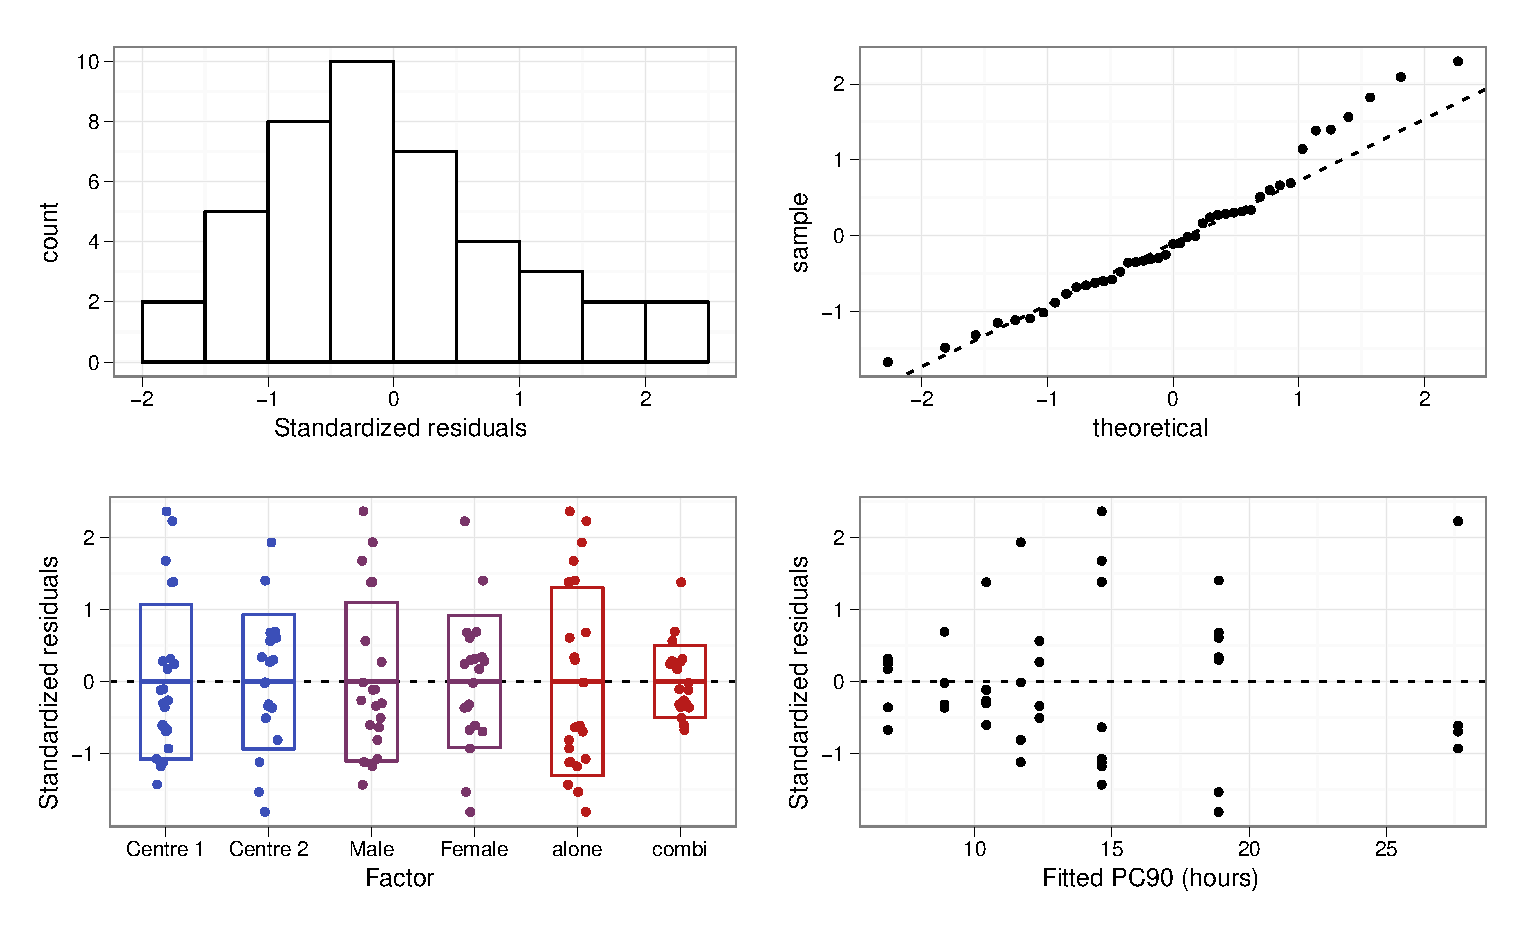
\includegraphics[width=6.5in]{aovloglinres.eps} 
\caption{Residuals from fitting a 3-way ANOVA model with interactions to PC90}
\label{aovloglinres}
\end{figure}
It can be seen that the residuals are approximately normally distributed, but perhaps slightly right skewed. In the plot of the residuals by experimental factor (bottom-left) the standard deviation of the residuals is shown, which when they are standardized, should be approximately 1 and independent of factor. We can see that this is so for centre and sex, but there is heteroscedasticity between treatments with the residuals for the single-drug treatment showing a larger variance than for the combined-drug treatment ($p<0.05$ under a Breusch-Pagan test for heteroscedasticity\cite{breusch} as implemented by the \texttt{bptest} \emph{R} function\cite{lmtest}). We can also see that the variance of the residuals increases with fitted PC90 value (bottom-right).

\subsection{Dealing with heteroscedasticity}
Least squares estimators are still unbiased under heteroscedasticity\cite{long}, but standard errors can be underestimated leading to incorrect inference.
\subsubsection*{Transforming the dependent variable}
If we apply a square-root transformation to PC90 we obtain the residuals for the ANOVA model shown in Figure \ref{aovsqrtres}.
\begin{figure}[p]
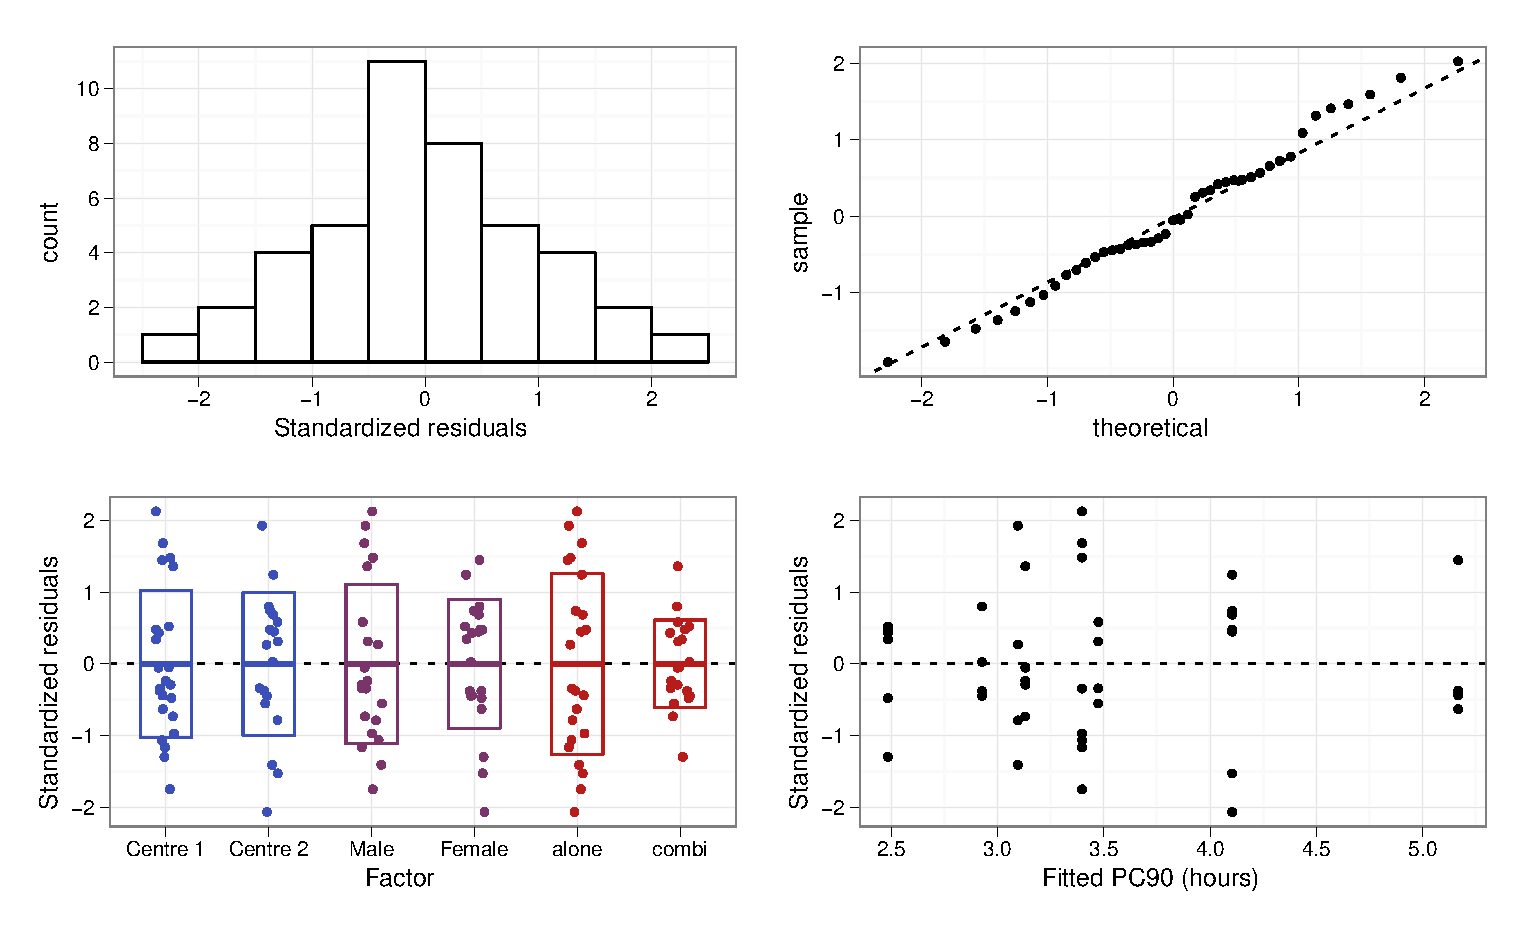
\includegraphics[width=6.5in]{aovsqrtres.eps} 
\caption{Residuals after applying a square-root transformation to the dependent variable}
\label{aovsqrtres}
\end{figure}
It can be seen that this transformation reduces the correlation of the variance of the residuals with fitted PC90. However, it can be seen that, even after our square-root transformation, the residuals for subjects on the combined treatment have a smaller variance than for those on the single treatment (Breusch-Pagan $p<0.05$).

Other transformations, such as logarithmic or square, did not prove as suitable as a square-root transformation. The Box-Cox method, whereby the transformation giving the highest likelihood is found, suggests transforming the dependent variable by raising it to the power 0.3 is optimal. This did not appear to give a noticeable improvement over the square-root transformation (power 0.5) in residual plots however. 

\subsubsection*{Weighted least-squares}
One common method of dealing with heteroscedastic residuals is to use weighted least-squares such that error term in model \ref{full} becomes
\begin{equation}
\epsilon\sim N(0,\sigma_{k}^2)\label{wls}
\end{equation}
where $\sigma_{1}^{2}$ is the variance of subjects on the single treatment and $\sigma_{2}^{2}$ is the variance of subjects on the combined treatment. This model is fitted by minimizing
\begin{equation*}
S=\sum_{ijkl} w_{k}(\mathrm{PC}90_{ijkl} - \widehat{\mathrm{PC}90_{ijk}})^{2}
\end{equation*}
where the weights $w_{k}=\sigma_{k}^{-2}$. The residuals from fitting this function using the \texttt{weights} parameter of the \emph{R} linear least-sqaures \texttt{lm} function are shown in Figure \ref{aovres}.
\begin{figure}[p]
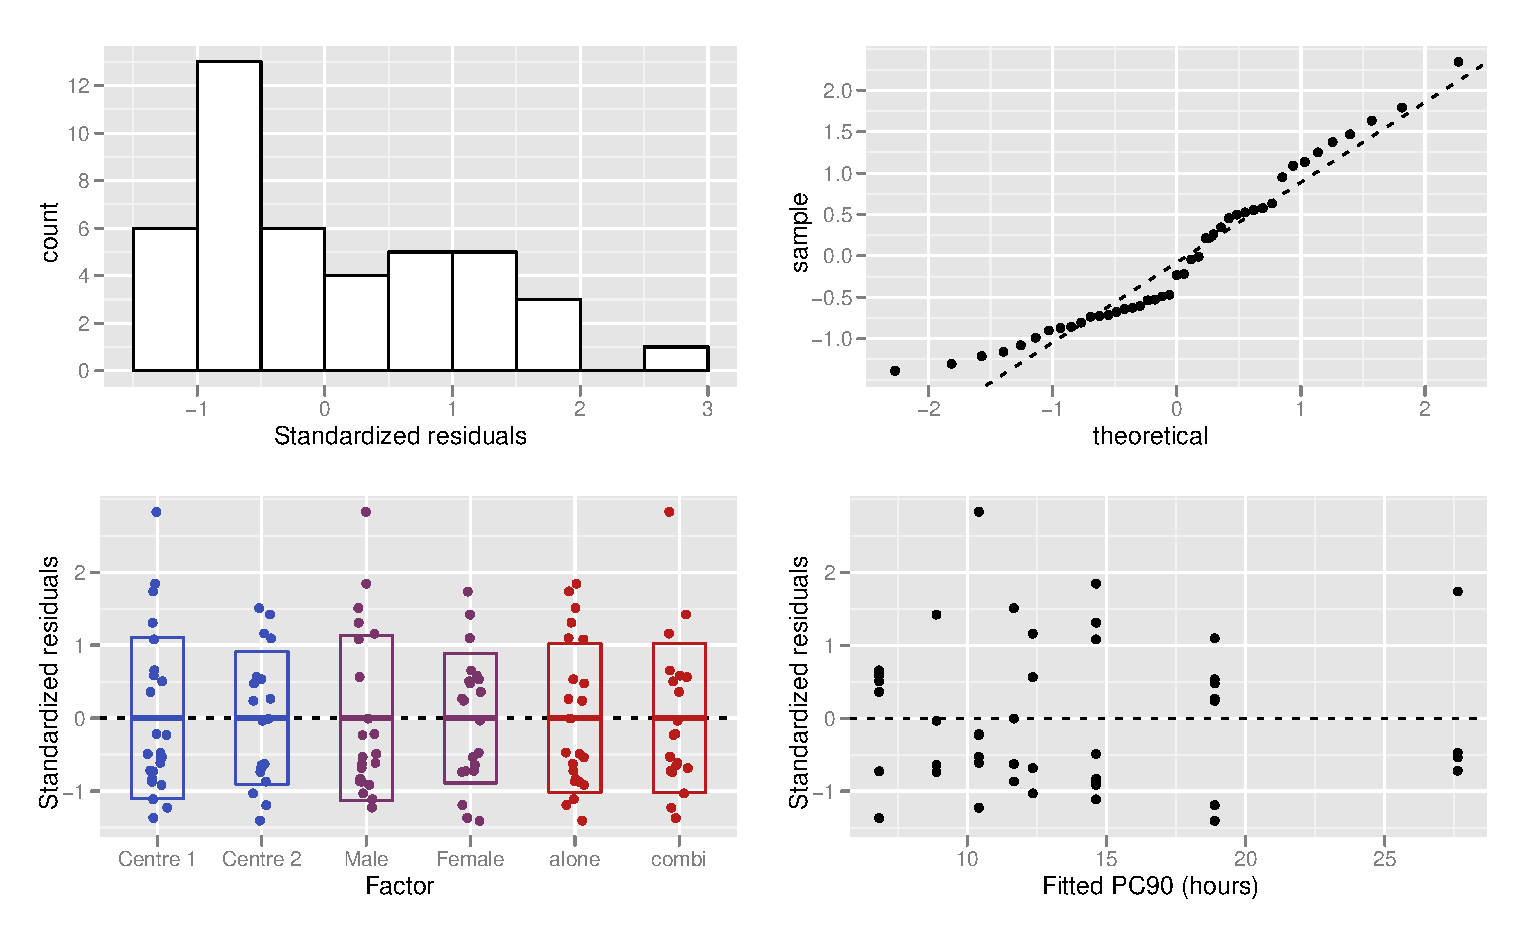
\includegraphics[width=6.5in]{aovresw.eps} 
\caption{Residuals after applying weighted least squares}
\label{aovresw}
\end{figure}
The residuals now have approximately equal variance with respect to factor and fitted PC90, but they appear to be right-skewed.

If we apply the square-root transformation followed by a weighted least-squares fit we obtain the residuals shown in Figure \ref{aovsqrtresw}.
\begin{figure}[h]
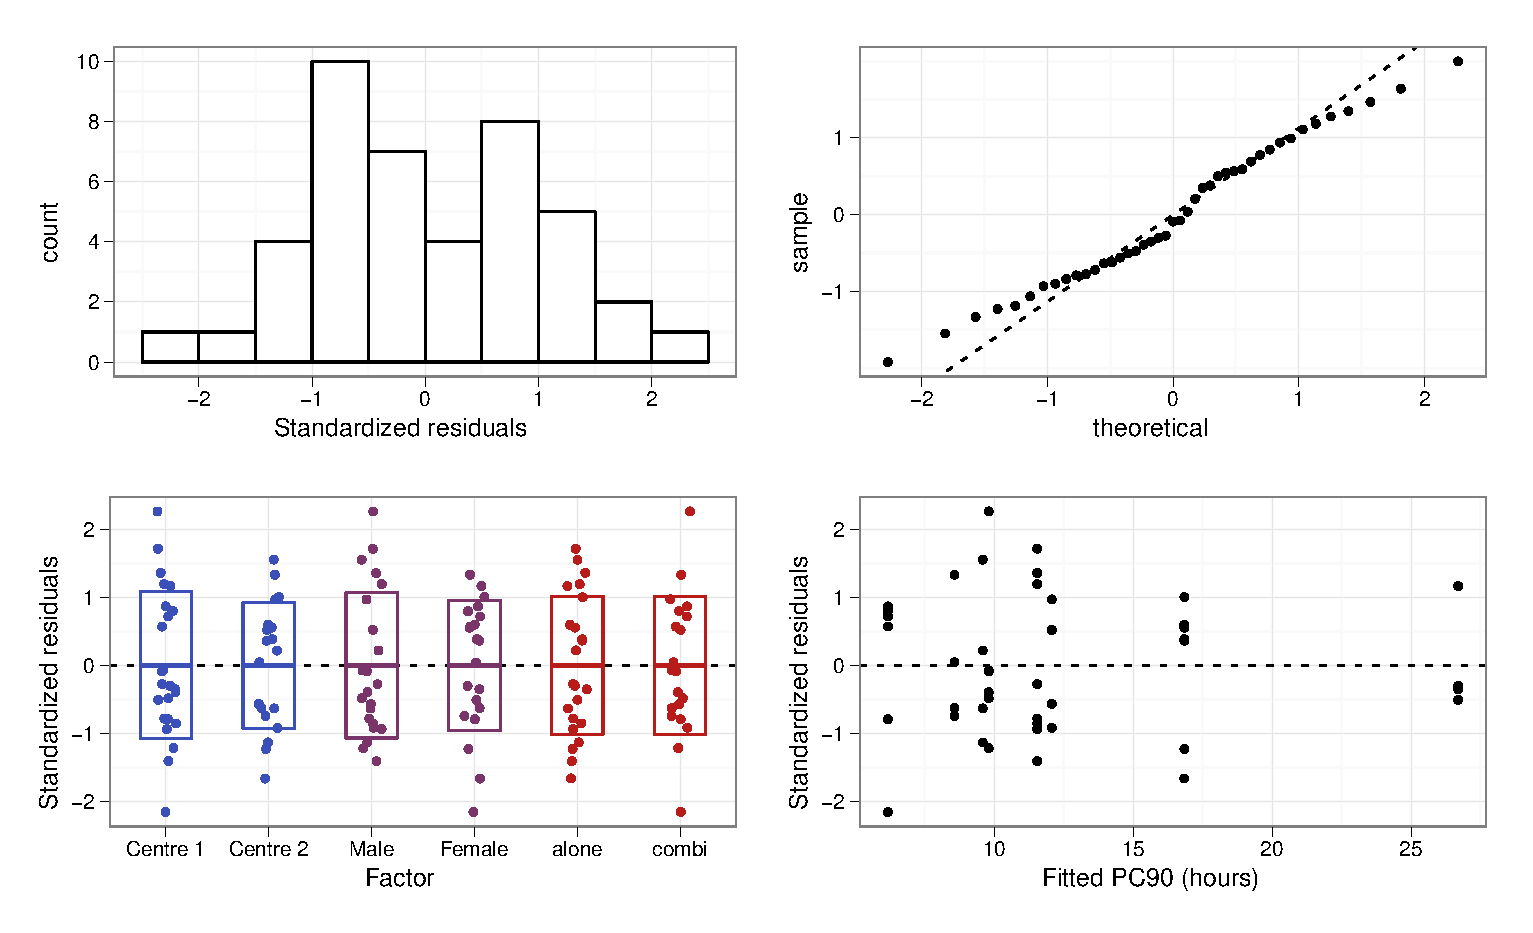
\includegraphics[width=6.5in]{aovsqrtresw.eps} 
\caption{Residuals after applying square-root transformation and weighted least squares}
\label{aovsqrtresw}
\end{figure}
This seems to give a more symmetric distribution of residuals but is perhaps a bit light-tailed.

Despite this, none of the distributions of residuals show evidence of significant departures from normality by a Shapiro-Wilk test and there also now seems to be no significant difference in the variance of the residuals between experimental groups.
\subsection{Model selection}
Now that we seem to have a transformation such that the assumptions of our model are met we can start to look at hypothesis tests on the experimental factors. Table \ref{aovwt} shows the results of the ANOVA analysis for model \ref{full} using  weighted least-squares. Table \ref{aovsqrtwt} shows the results for the model using a square root transformation and weighted least-squares.
\begin{table}[h]
\centering
\caption{ANOVA table for full model fitted by weighted least-squares}\label{aovwt}
\begin{tabular}{l|rrrrrl}
Source&Sum Sq.&df&Mean Sq.&$F$&P($>F$)\\
\hline
$Centre$     &                0.631  &1& 0.631 & 0.654 &0.424&\\
$Sex$        &              0.972  &1& 0.972 & 1.01 &0.322\\
$Treatment$  &            7.85  &1& 7.85  &8.14 &0.007 &**\\
$Centre\times Sex$ &             0.001 &1&  0.001 & 0.001 &0.975&\\
$Centre\times Treatment$ &        0.511  &1& 0.511 & 0.530 &0.472&\\
$Sex\times Treatment$     &     5.21  &1& 5.21 & 5.40 &0.026 &* \\
$Centre\times Sex\times Treatment$ &   0.239 &1&  0.239 & 0.247& 0.622&\\
$Residuals$      &    33.76 &35&  0.965  &&&\\
\hline
Total&49.17&42&&&
\end{tabular}\\
$*<0.05\quad\quad**<0.01$
\end{table}
\begin{table}[h]
\centering
\caption{ANOVA table for full model with square-root transformation fitted by weighted least-squares}\label{aovsqrtwt}
\begin{tabular}{l|rrrrrl}                   
Source&Sum Sq.&df&Mean Sq.&$F$&P($>F$)\\
\hline
$Centre$     &                0.834 &1&  0.834 & 0.882 & 0.354 &\\    
$Sex$        &               0.630 &1&  0.630 & 0.666 & 0.420 &\\  
$Treatment$  &            4.89 &1&  4.89 &  5.17 & 0.029& *\\
$Centre\times Sex$ &             0.003 &1& 0.003 & 0.003 & 0.956&\\
$Centre\times Treatment$ &        0.523 &1&  0.523 & 0.553 & 0.462&\\
$Sex\times Treatment$     &     5.94 &1& 5.94 & 6.28 & 0.017& *\\
$Centre\times Sex\times Treatment$ &   0.271 &1&  0.271 & 0.287 & 0.596&\\
$Residuals$      &    33.118 &35&  0.946 &&&\\
\hline
Total&46.21&42&&&
\end{tabular}\\
$*<0.05$
\end{table}
It can be seen that there is no evidence to reject the hypothesis that the centre has no effect on the clearance time. 
\subsubsection*{Non-parametric check on $p$-values}
We checked that our residuals were approximately normally distributed and homoscedastic and so our hypothesis tests and standard errors, based on these assumptions, should be accurate. However, we can perform an additional non-parametric validation by resampling methods.

If we randomize the clearance times among the 43 patients and then refit our model and calculate the $F$ statistic for each randomization we can construct the empirical distribution of the statistic and obtain $p$-values from this. This was done using 10,000 samples and the results are shown in Table \ref{aovresamp}, where the $p$-value from the F distribution ($P_{F}$), the empirical distribution obtained by randomising ($P_{rand}$) and the empirical bootstrap distribution ($P_{boot}$), whereby instead of randomising the 43 values, we resample with replacement.
\begin{table}[h]
\centering
\caption{Comparison of parametric $p$-values and $p$-values from resampling}\label{aovresamp}
\begin{tabular}{l|rrrr|rrrrl}
&\multicolumn{4}{c}{Weighted LSQ}&\multicolumn{4}{c}{Sqrt weighted LSQ}&\\                   
Source&$F$&$P_{F}$&$P_{rand}$&$P_{boot}$&$F$&$P_{F}$&$P_{rand}$&$P_{boot}$&\\
\hline
$Centre$     						& 0.654 & 0.424 & 0.536 & 0.547     	& 0.882 & 0.354 & 0.434 & 0.437 &\\    
$Sex$        						& 1.01   & 0.322 & 0.440 & 0.446     	& 0.666 & 0.420 & 0.498 & 0.500 &\\  
$Treatment$ 						& 8.14   & 0.007 & 0.001 & 0.002     	& 5.17   & 0.029 & 0.012 & 0.012 &*\\
$Centre\times Sex$ 					& 0.001 & 0.975 & 0.982 & 0.981     	& 0.003 & 0.956 & 0.962& 0.964 &\\
$Centre\times Treatment$			& 0.530 & 0.472 & 0.322 & 0.328	& 0.553 & 0.462 & 0.381& 0.375 &\\
$Sex\times Treatment$     			& 5.40   & 0.026 & 0.003 & 0.003	& 6.28   & 0.017 & 0.005& 0.005 &*\\
$Centre\times Sex\times Treatment$	& 0.247 & 0.622 & 0.482 & 0.491	& 0.287 & 0.596 & 0.507& 0.516 &\\
\hline
\end{tabular}
\end{table}

It can be seen that the $p$-values obtained by the parametric and non-parametric methods are in general agreement, although the F test seems more conservative than the non-parametric tests. In all 3 cases it can be seen that there is no evidence to reject the hypothesis that the effect of the centre is negligible.
\subsubsection*{Fitting a reduced model}
As the effect of centre is negligible we refit the data with the reduced model
\begin{equation}
\sqrt{\mathrm{PC}90_{jk}}=\mu+S_j+T_k+(ST)_{jk}+\epsilon_{ijk}\quad\quad\epsilon\sim N(0,\sigma_{k}^2)\label{reduced}
\end{equation}
using weighted least-squares. The residuals for this fit are shown in Figure \ref{aov2rwt}.
\begin{figure}[h]
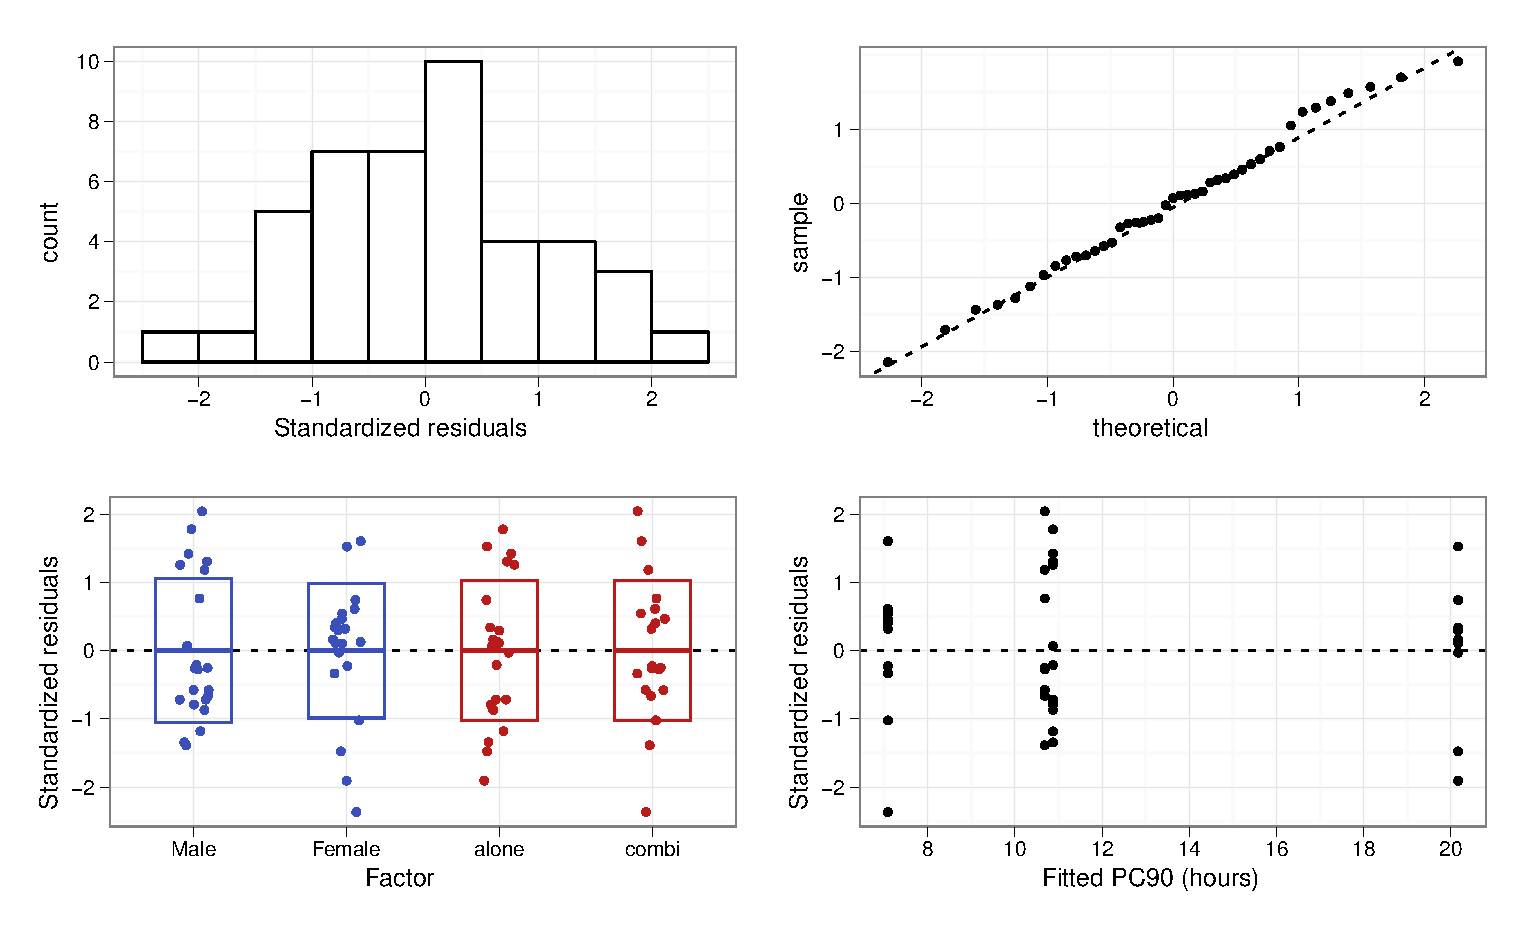
\includegraphics[width=6.5in]{aov2rwt.eps} 
\caption{Residuals for the reduced model}
\label{aov2rwt}
\end{figure}
It can be seen that they are approximately normal and homoscedastic. The ANOVA table for this model is shown in Table \ref{aovreduced}, where the results are essentially the same as for the full model with some variation in the sex and treatment sums of squares due to the design matrix not being orthogonal.
\begin{table}[h]
\centering
\caption{ANOVA table for the reduced model}\label{aovreduced}
\begin{tabular}{l|rrrrrl}
Source&Sum Sq.&df&Mean Sq.&$F$&P($>F$)\\
\hline
$Sex$				& 0.032 & 1 & 0.032 & 1.58 & 0.217 & \\
$Treatment$			& 0.096 & 1 & 0.096 & 4.78 & 0.035 & *\\
$Sex\times Treatment$	& 0.097 & 1 & 0.097 & 4.83 & 0.034 & *\\
$Residuals$			& 0.784 & 1 & 0.020 &&&\\
\hline
Total&83.66&42&&&
\end{tabular}\\
$*<0.05$
\end{table}

The fitted coefficients for the reduced model are shown in Table \ref{coefreduced}.
\begin{table}[h]
\centering
\caption{Fitted coefficients for the reduced model}\label{coefreduced}
\begin{tabular}{l|rrrrl}
Factor levels&Coefficient&S.E.&$t$&P($>|t|$)\\
\hline
Male, single treatment ($\mu$)			& 3.30 & 0.52 & 6.29 &  $2\times 10^{-7}$ & *** \\
$\Delta$Female, single treatment		& 1.19 & 0.76 & 1.57 & 0.124 & \\
$\Delta$Male, combined treatment		& -0.029 & 0.57 & -0.051 & 0.96 & \\
$\Delta$Female, combined treatment	& -1.80 & 0.82 & -2.20 & 0.034 & *\\
\hline
\end{tabular}\\
$*<0.05\quad\quad***<0.0001$\\
Residual standard error: 0.14, Adjusted $R^{2}$: 0.16
\end{table}
With the corner-point constraint used only the male, single-treatment coefficient is absolute, the other 3 are the change in clearance time from this (indicated by $\Delta$). It can be seen that there is evidence to reject the hypothesis that the difference in clearance times between male, single treatment subjects and 
\subsection{Inference for Clearance Times}
Bearing in mind that a square-root transformation was used, we have from Table \ref{coefreduced}:
%\begin{itemize}
%\item The mean clearance time for male patients on the single treatment is $3.30^{2}=10.88$ hours with a 95\% confidence interval of ($2.54^{2},\ 4.05^{2})=(6.47,\ 16.41)$ hours.
%\item There is no evidence to reject the hypothesis that there is no difference between mean clearance times for male subjects on the single and combined treatments.
%\item Female subjects on the single treatment have a mean clearance time of $(3.30+1.19)^{2}=20.16$ hours with a 95\% confidence interval of (13.72, 27.85) hours.
%\item Female subjects on the combined treatment have a mean clearance time of $(3.30+1.19-0.029-1.80)^{2}=7.09$ hours with a 95\% confidence interval of (3.37, 12.16) hours.
%\end{itemize}
\begin{table}[h]
\centering
\caption{Fitted coefficients for the reduced model}\label{coefreduced}
\begin{tabular}{|l|c|c|}
\hline
&Clearance time PC90&95\% conf. int.\\
Factor levels&(hrs:mins)&(hrs:mins)\\
\hline
Male, single treatment 		& 10:52 & (5:00, 19:00) \\
Female, single treatment		& 20:10 & (11:26,  31:20) \\
Male, combined treatment	& 10:41 & (7:59, 13:46) \\
Female, combined treatment	& 7:05 & (4:56, 9:38) \\
\hline
\end{tabular}
\end{table}

\clearpage
\section{Dependence of clearance time on initial variables}
\begin{figure}[h]
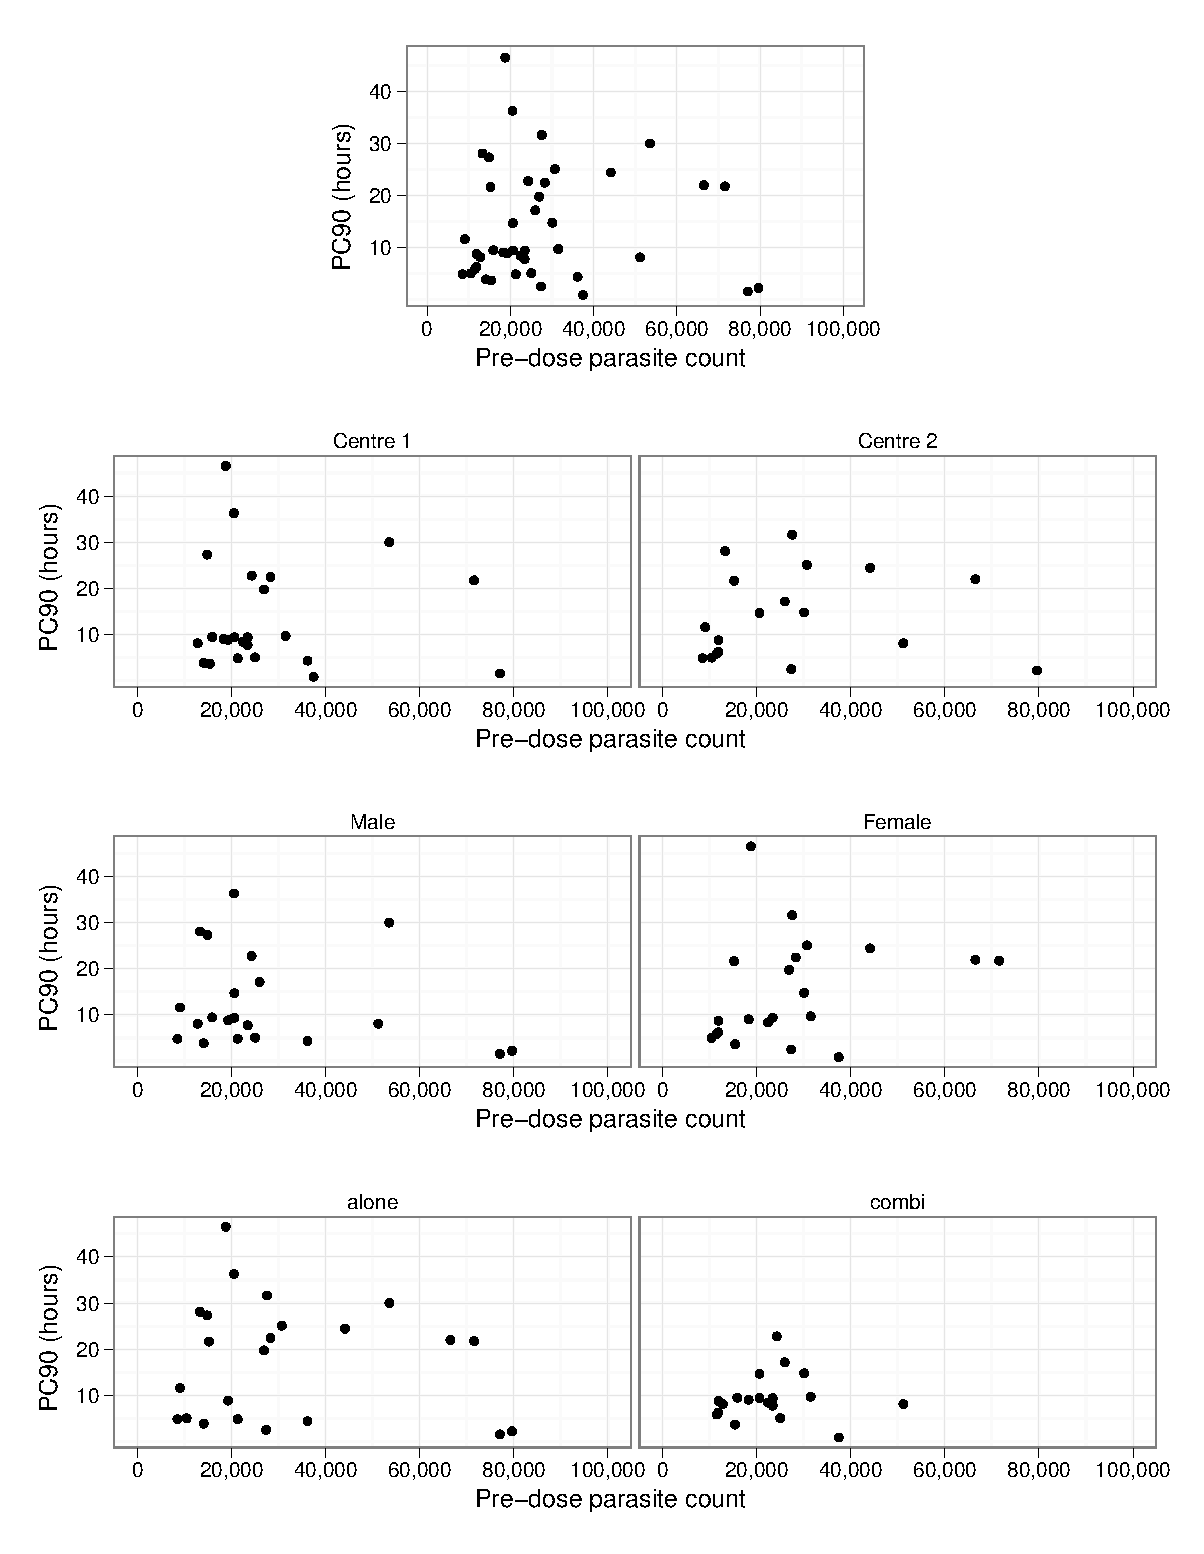
\includegraphics[width=6.5in]{predose-ancova.eps} 
\caption{Dependence of clearance time on pre-dose parasite count}
\label{predose-ancova}
\end{figure}
\begin{figure}[h]
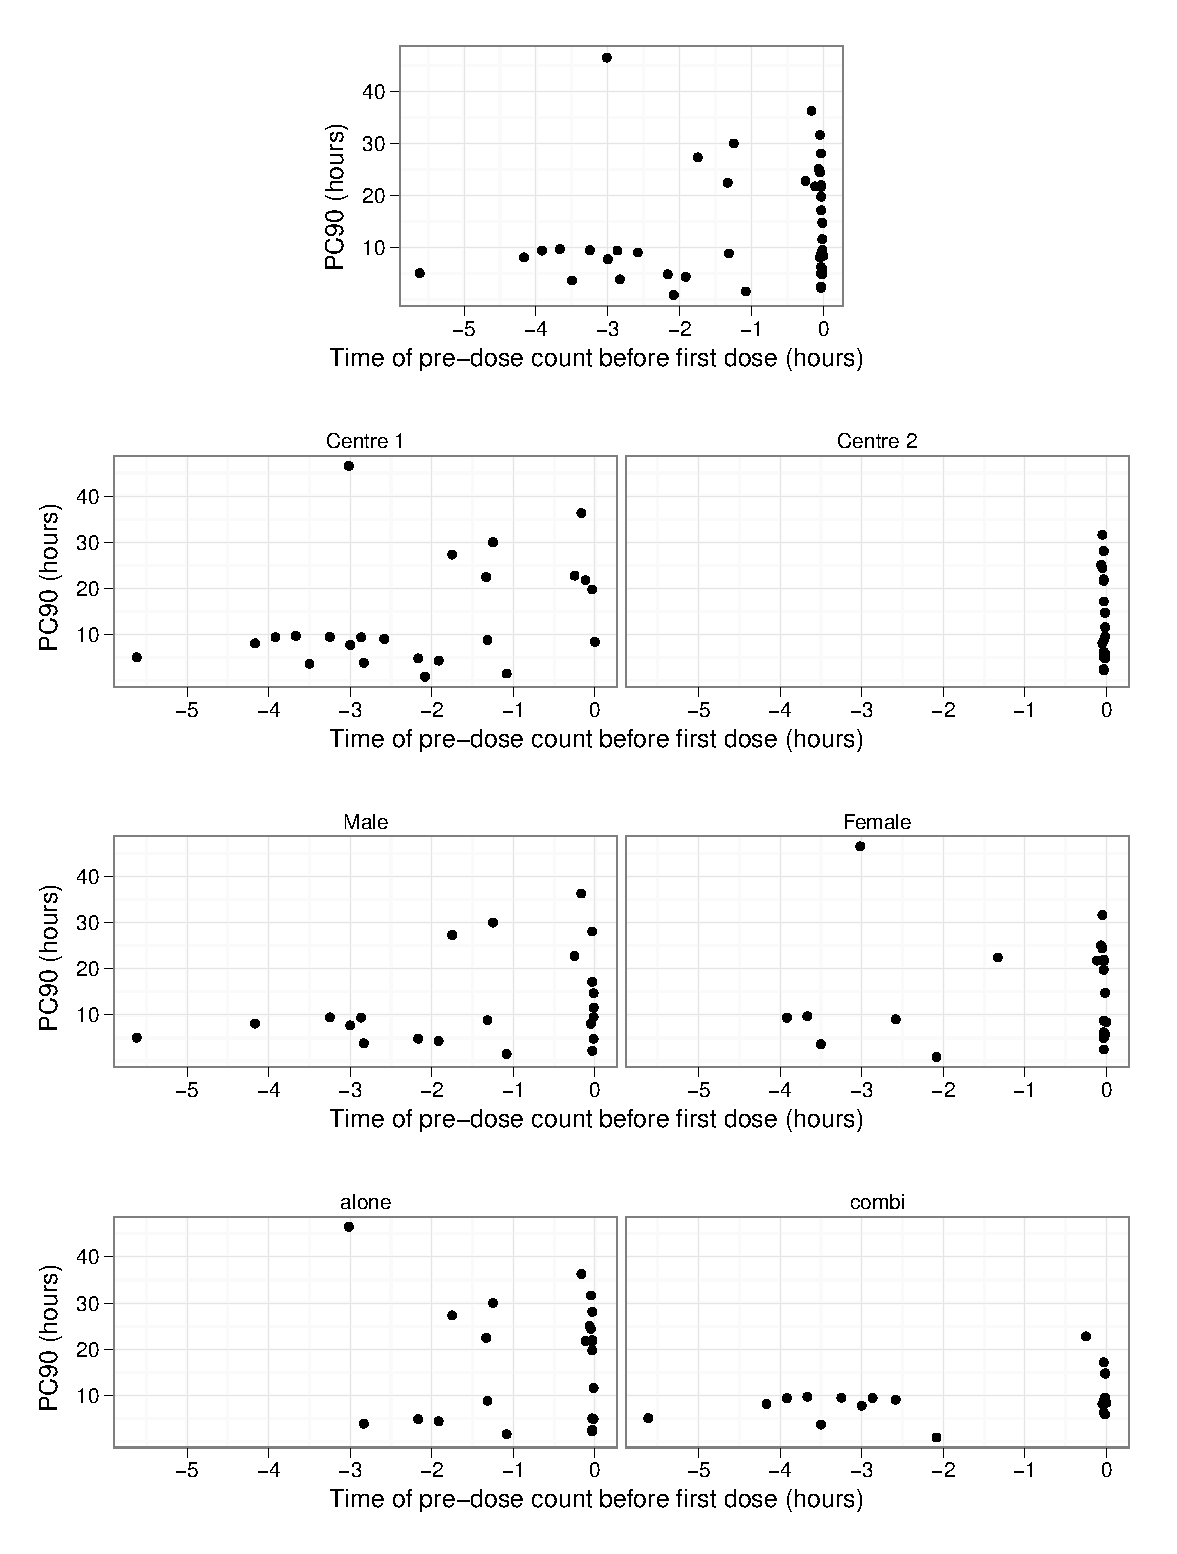
\includegraphics[width=6.5in]{pretime-ancova.eps} 
\caption{Dependence of clearance time on the time before first dose that the pre-dose parasite count was recorded}
\label{predtime-ancova}
\end{figure}